\documentclass{altsu-report}
\linespread{1,15}
\title{Автоматизация решения CAPTCHA в текстовом формате}
\author{А.\,В.~Лаптев}
\groupnumber{5.306М}
\GradebookNumber{1337}
\supervisor{А.\,В.~Калачев}
\supervisordegree{доц. каф. ВТиЭ}
\ministry{Министерство науки и высшего образования}
\country{Российской Федерации}
\fulluniversityname{ФГБОУ ВО Алтайский государственный университет}
\institute{Институт цифровых технологий, электроники и физики}
\department{Кафедра вычислительной техники и электроники}
\departmentchief{В.\,В.~Пашнев}
\departmentchiefdegree{к.ф.-м.н., доцент}
\shortdepartment{ВТиЭ}
\abstractRU{
Данная научно-исследовательская работа посвящена разработке и исследованию методов автоматического распознавания символов на текстовых CAPTCHA с использованием современных подходов в области машинного обучения и компьютерного зрения. Основной целью проекта является создание эффективной нейросетевой модели, способной с достаточной точностью интерпретировать текстовые CAPTCHA-изображения, содержащие искаженные или зашумленные символы, с целью автоматизации ввода данных на web-ресурсах. Это актуально при разработке систем автоматизированного тестирования web-приложений, где CAPTCHA представляет собой препятствие для непрерывного выполнения тестов. В ходе работы были рассмотрены и реализованы различные архитектуры нейронных сетей, включая сверточно-рекуррентные сети (CRNN) и модели типа Seq-to-Seq, а также проведено сравнение с традиционными методами OCR, в частности, системой Tesseract. Для обучения и валидации моделей использовались синтетические датасеты CAPTCHA. Работа выполнена с использованием фреймворка TensorFlow и языка программирования Python. Полученные результаты демонстрируют достаточную точность распознавания и подтверждают перспективность использования нейросетевых подходов для автоматизации решения текстовых CAPTCHA.
}
\keysRU{CAPTCHA, нейронная сеть, TensorFlow, Python, OCR, Tesseract, CRNN, Seq-to-Seq}

\date{\the\year}

% Подключение файлов с библиотекой.
\addbibresource{graduate-students.bib}

\begin{document}

\maketitle

\setcounter{page}{2}
\makeabstract
\tableofcontents

\chapter*{Введение}
\addcontentsline{toc}{chapter}{Введение}

CAPTCHA давно является стандартным инструментом для защиты веб-ресурсов от спама, автоматизированных ботов и нежелательного извлечения данных. Большинство современных сайтов и веб-приложений используют данную технологию в различных сценариях, включая регистрацию пользователей, подтверждение действий на сайте и защиту от автоматизированных атак.

Несмотря на развитие технологий CAPTCHA, включая невидимые для пользователя решения, текстовая CAPTCHA и её различные модификации остаются широко распространёнными. В связи с этим автоматизация процесса решения таких CAPTCHA сохраняет актуальность.

Автоматизированное распознавание текстовых CAPTCHA позволяет значительно снизить необходимость ручного тестирования веб-приложений, что, в свою очередь, повышает скорость и эффективность тестирования. Кроме того, подобные методы могут использоваться для анализа надёжности внедрённых CAPTCHA, выявления их слабых мест и повышения безопасности веб-приложений, например, за счёт комбинирования нескольких методов защиты.

Цель работы -- разработать, реализовать и протестировать программу для автоматизированного распознавания текстовых CAPTCHA.

Для достижения поставленной цели необходимо решить следующие задачи:
\begin{enumerate}
    \item изучить принципы реализации текстовых CAPTCHA на основе открытых источников (допустимые символы, применяемые искажения);
    \item выбрать архитектуру нейронной сети, наиболее подходящую для распознавания CAPTCHA;
    \item подготовить датасет изображений CAPTCHA с учётом возможных искажений;
    \item обучить нейронную сеть с достаточной точностью;
    \item протестировать модель на тестовом наборе данных и оценить её эффективность.
\end{enumerate}

\chapter{Обзор текстовых CAPTCHA и методов автоматизации их решения}

\section{Современная реализация текстовых CAPTCHA}

Современные текстовые CAPTCHA обычно состоят из букв и цифр. Зачастую используются символы латинского алфавита (как прописные, так и строчные) и цифры от 0 до 9. Но обычно реализации исключают символы, которые могут быть легко перепутаны, например, буквы <<O>> и цифру <<0>>, буквы <<I>> и <<l>> и тому подобное. Рекомендуемый набор символов в генераторах на некоторых CRM платформах выглядит следующим образом: ABCDEFGHJKLMNPQRSTWXYZ23456789~\cite{Bitrix}.

Длина последовательности символов в CAPTCHA обычно составляет от 4 до 8 символов, что обеспечивает баланс между удобством для пользователя и безопасностью, однако конкретная длина может варьироваться в зависимости от требований системы безопасности.

Для усложнения автоматического распознавания текстовые CAPTCHA подвергаются различным искажениям~\cite{HabrCaptcha, Proglib}:
\begin{enumerate}
    \item геометрические искажения: символы могут быть искажены, повернуты или наклонены, что затрудняет их распознавание автоматическими системами;
    \item перекрытие символов: символы могут быть расположены близко друг к другу или даже перекрываться, что усложняет их сегментацию и последующее распознавание;
    \item добавление шума: на изображение могут быть добавлены различные шумы, такие как линии, точки или круги, чтобы затруднить распознавание символов;
    \item сложные фоны: использование фонов с различными цветами или узорами, что делает выделение символов более сложным;
    \item нелинейные искажения: применение нелинейных трансформаций к символам, что делает их форму менее предсказуемой для автоматических систем распознавания.
\end{enumerate}

Эти методы направлены на повышение сложности автоматического распознавания CAPTCHA, сохраняя при этом относительную легкость распознавания для человека. 

\section{Подготовка датасета с изображениями и выбор модели нейронной сети}

Качество используемого датасета оказывает существенное влияние на итоговую точность работы модели. Для эффективного обучения необходимо, чтобы набор данных соответствовал следующим требованиям:

\begin{enumerate}
    \item достаточное количество изображений для каждого символа, что обеспечивает статистическую устойчивость модели;
    \item разнообразие данных, включающее:
    \begin{enumerate}
        \item различные углы наклона символов;
        \item вариативность написания символов и их искажения;
        \item наличие побочных визуальных элементов, создающих препятствия для распознавания;
        \item использование различных шрифтов.
    \end{enumerate}
    \item переменная длина последовательностей символов, что позволяет модели адаптироваться к разным формам CAPTCHA.
\end{enumerate}

Включение указанных факторов способствует обучению модели на более широком спектре признаков, что, в свою очередь, повышает её способность к обобщению на ранее невидимых данных.

Поскольку в открытом доступе отсутствует достаточное количество данных для формирования сбалансированного датасета, было принято решение о генерации синтетических изображений с использованием специализированных библиотек. В качестве основного инструмента выбрана библиотека captcha на языке Python, обладающая необходимым функционалом для создания изображений CAPTCHA с заданными параметрами. Данная библиотека поддерживает генерацию изображений с пользовательскими шрифтами и различными эффектами искажений, что исключает необходимость привлечения дополнительных инструментов.

Исходный код генератора синтетических CAPTCHA представлен в Приложении (листинг~\ref{code:gen-dataset}).

После создания изображений все они прошли этапы предобработки, направленные на улучшение качества данных и повышение эффективности обучения модели. Предобработка включала следующие этапы:

\begin{enumerate}
    \item преобразование изображений в градации серого для уменьшения количества каналов и снижения вычислительной нагрузки;
    \item бинаризация изображений с целью получения контрастного представления символов (белый текст на черном фоне);
    \item удаление шумов и фона с использованием морфологических операций, в частности, дилатации.
\end{enumerate}

Исходный код обработчика изображений и формирования датасета представлен в Приложении (листинг~\ref{code:preprocessing}, листинг~\ref{code:tf-dataset}).

Примеры сгенерированных и предобработанных CAPTCHA приведены на рисунке ниже:

\begin{figure}[H]
    \centering
    \begin{minipage}[h]{0.45\linewidth}
        \center{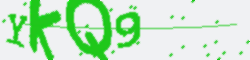
\includegraphics[width=1\linewidth]{imgs/YKQ9.png}} \\
    \end{minipage}
    \begin{minipage}[h]{0.45\linewidth}
        \center{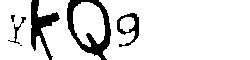
\includegraphics[width=1\linewidth]{imgs/out.png}} \\
    \end{minipage}
    \caption{Изображение сгенерированной CAPTCHA и результат обработки.}
    \label{fig:example-captcha}
\end{figure}

\vspace{-0.7cm}

Для распознавания текста с переменной длиной последовательности в задачах CAPTCHA наиболее часто применяются следующие архитектуры нейронных сетей:

\begin{enumerate}
    \item оптическое распознавание символов (OCR);
    \item рекуррентные сверточные нейронные сети (CRNN);
    \item архитектуры последовательного обучения (Seq-to-Seq).
\end{enumerate}

С целью выбора наиболее эффективной модели были реализованы и протестированы все указанные подходы, после чего была выбрана архитектура, обеспечивающая наилучшую точность предсказаний.

Для обучения моделей был сформирован датасет из 100 000 изображений CAPTCHA, содержащих случайные последовательности символов длиной от 4 до 7. Такой объем данных позволяет добиться высокой обобщающей способности модели и снизить вероятность переобучения.

\section{Оптическое распознавание символов (OCR Tesseract)}

Изначально предполагалась реализация модели с использованием OCR, поскольку такие системы изначально разрабатывались для задач оптического распознавания текста. В качестве конкретной модели был выбран Tesseract.

Tesseract является одной из наиболее популярных систем OCR с открытым исходным кодом. Tesseract поддерживает более 100 языков, включая сложные письменности~\cite{Klippa}. В версии 4.0 в модель была интегрирована нейронная сеть на основе долговременной краткосрочной памяти (LSTM), что позволило существенно повысить точность распознавания, особенно при обработке сложных шрифтов и рукописного текста~\cite{GitTesseract}.

Для решения поставленной задачи предполагалось использовать предобученную модель Tesseract и дообучить её на специализированном датасете, содержащем изображения CAPTCHA с характерными искажениями. Однако в ходе экспериментов было установлено, что точность распознавания последовательностей символов целиком составляла 0\%, а точность для отдельных символов оказалась крайне низкой. Это связано с тем, что архитектура Tesseract недостаточно устойчива к искажениям, характерным для CAPTCHA, таким как деформация символов, наложение шумов и изменение углов наклона~\cite{TrainTesseract}.

Таким образом, было принято решение отказаться от использования Tesseract в пользу более адаптированных к данной задаче моделей, таких как сверточные рекуррентные нейронные сети (CRNN) или модели последовательного обучения (Seq-to-Seq), обладающие высокой устойчивостью к вариативности и искажениям, характерным для CAPTCHA.

\section{Рекуррентные сверточные нейронные сети (CRNN)}

Сверточно-рекуррентные нейронные сети (CRNN) представляют собой гибридную архитектуру, сочетающую в себе возможности сверточных нейронных сетей (CNN) и рекуррентных нейронных сетей (RNN). Данный подход используется в задачах, связанных с обработкой последовательных данных, таких как распознавание текста, речь и видео~\cite{CRNNHabr}.

Основное преимущество CRNN заключается в способности CNN-части извлекать пространственные признаки из изображений, тогда как RNN-часть позволяет учитывать временные зависимости между последовательными фрагментами данных~\cite{CRNNBook}.

Разработанная модель CRNN для распознавания CAPTCHA включает в себя три ключевых блока:
\begin{enumerate}
    \item сверточный блок (CNN): предназначен для выделения признаков из изображений CAPTCHA. Включает в себя три последовательных сверточных слоя, а также методы нормализации и уменьшения размерности признакового пространства;
    \item рекуррентный блок (RNN): использует двунаправленные слои GRU, позволяющие модели учитывать зависимость между последовательными символами в CAPTCHA;
    \item выходной слой: полносвязный, который выполняет классификацию каждого символа в последовательности.
\end{enumerate}

В Приложении (листинг~\ref{code:crnn}) представлена реализация CRNN-модели на языке Python с использованием библиотеки TensorFlow/Keras:

В данной архитектуре применяются слои Dropout для регуляризации, также используется l2-регуляризация, BatchNormalization для ускорения обучения и повышения устойчивости модели, а также функция softmax для предсказания классов символов.

После обучения данной модели результаты оказались превосходящими показатели OCR, однако все же не достигли удовлетворительного уровня. В частности, точность распознавания всей последовательности символов не превышала 10\%, тогда как точность классификации отдельных символов составляла около 70\%.

\section{Архитектура последовательного обучения (Seq-to-Seq)}

Модели последовательного преобразования (Seq-to-Seq) широко применяются для задач, связанных с обработкой последовательностей переменной длины. Они используются в таких областях, как машинный перевод, распознавание речи и анализ текстов~\cite{Seq2Seq}. Данные модели основаны на архитектуре энкодера-декодера, где первый модуль кодирует входную последовательность в скрытое представление, а второй декодирует его в выходную последовательность.

Одним из ключевых элементов Seq2Seq является механизм внимания, который позволяет декодеру динамически фокусироваться на различных частях входной последовательности при генерации выходных символов~\cite{Seq2SeqBook}. Этот подход особенно полезен для распознавания CAPTCHA, так как символы в изображениях могут иметь разную ориентацию и степень искажения.

Кодировщик, в данной модели принимает входное изображение CAPTCHA и преобразует его в компактное представление. Архитектура кодировщика включает:
\begin{enumerate}
    \item четыре сверточных блока, слои пакетной нормализации и слои подвыборки для понижения размерности входных данных;
    \item глобальный усредненный слой для получения векторного представления изображения;
    \item полносвязный слой для финального представления скрытого состояния;
    \item рекуррентный слой для кодирования последовательности, возвращающий последнее скрытое состояние кодировщика.
\end{enumerate}

Декодировщик выполняет пошаговую генерацию выходной последовательности, используя скрытое состояние кодировщика. В архитектуру декодировщика входят:
\begin{enumerate}
    \item входной слой для последовательности токенов;
    \item слой вложения, который преобразует входные токены в векторные представления;
    \item рекуррентный слой, обрабатывающий последовательность с учетом скрытого состояния кодировщика;
    \item механизм внимания, который позволяет декодеру учитывать релевантные части входного изображения;
    \item полносвязный слой с функцией активации softmax для предсказания вероятностей символов.
\end{enumerate}

Полная архитектура модели реализована в TensorFlow/Keras и реализация модели приведена в Приложении (листинг~\ref{code:seq2seq}).

На начальных этапах экспериментов предложенная Seq-to-Seq-модель показала наилучшие результаты среди рассмотренных вариантов. В отличие от OCR- и CRNN-моделей, данная архитектура смогла достичь более высокой точности распознавания последовательностей символов, что обусловлено применением механизма внимания. Дальнейшая работа с моделью была сосредоточена на её оптимизации и улучшении параметров обучения.

\chapter{Тестирование Seq-to-Seq модели и анализ результатов}

Как было установлено в предыдущих разделах, модель последовательного преобразования (Seq-to-Seq) продемонстрировала наилучшие результаты среди рассмотренных архитектур. Следующим этапом работы являлась оптимизация параметров модели, включая веса и коэффициенты регуляризации, с целью ускорения сходимости, минимизации риска переобучения и повышения точности распознавания целевых последовательностей.

Для проведения экспериментов исходный набор данных, содержащий 100 000 изображений, был случайным образом перемешан и разделён на три подмножества: обучающее, тестовое и валидационное в соотношении 80:10:10. Обучающая выборка использовалась непосредственно для обучения модели, валидационная — для контроля качества процесса обучения на каждой эпохе, а тестовая — для окончательной оценки модели на данных, с которыми она ранее не сталкивалась. В качестве основных метрик качества модели использовались функция потерь (loss) и точность (accuracy), рассчитываемая для каждого символа последовательности.

В процессе многократного обучения были экспериментально определены оптимальное количество эпох и значения гиперпараметров, обеспечивающие эффективное снижение функции потерь до приемлемых значений. Скрипт для построения необходимых для анализа графиков представлен в Приложении (листинг~\ref{code:test-model}). График сходимости функции потерь представлен на рис.~\ref{fig:loss}.

\begin{figure}[H]
    \centering
    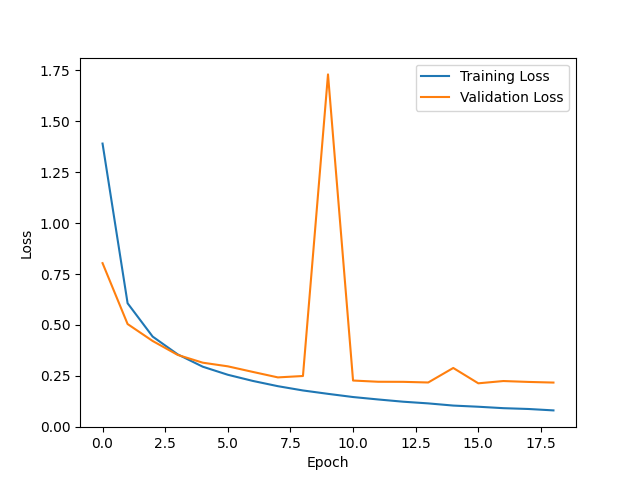
\includegraphics[width=0.65\linewidth]{imgs/Model_loss.png}
    \caption{График изменения значений функции потерь в процессе обучения.}
    \label{fig:loss}
\end{figure}

\vspace{-0.7cm}

Для предотвращения переобучения использовался механизм ранней остановки, согласно которому обучение прекращалось при отсутствии уменьшения значения функции потерь на валидационной выборке в течение трёх последовательных эпох. В данном эксперименте обучение завершилось на 18-й эпохе. На графике видно, что функция потерь стабилизировалась после 10 эпохе, поэтому 10 эпоха является балансом между точностью распознавания последовательностей и скоростью обучения модели.

Анализ графика сходимости функции потерь показывает наличие резкого увеличения её значения на 9-й эпохе, что может быть обусловлено следующими факторами:

\begin{enumerate}
    \item перемешивание данных перед каждой эпохой могло привести к образованию несбалансированной выборки, содержащей значительное число сложных примеров.
    \item динамическое изменение скорости обучения, осуществляемое с помощью механизма регулирования скорости обучения (learning rate scheduler), могло повлиять на изменение функции потерь.
\end{enumerate}

Окончательная точность распознавания отдельных символов составила 0.9263.

После подбора оптимальных значений гиперпараметров модель была сохранена и протестирована на валидационной выборке. Точность распознавания последовательностей различной длины представлена в таблице~\ref{tab:probability}.

\begin{table}[H]
    \centering
    \caption{Точность предсказаний для последовательностей различной длины.}
    \begin{tabular}{|l|l|}
        \hline
        Длина последовательности & Точность распознавания \\
        \hline
        4 символа & 0.9305 \\
        \hline
        5 символов & 0.7450 \\
        \hline
        6 символов & 0.4575 \\
        \hline
        7 символов & 0.1915 \\
        \hline
    \end{tabular}
    \label{tab:probability}
\end{table}

\vspace{-0.7cm}

Также была построена матрица ошибок, позволяющая проанализировать частоту и характер ошибок модели при классификации различных классов. Данная матрица приведена на рис.~\ref{fig:cm}.

\begin{figure}[H]
    \centering
    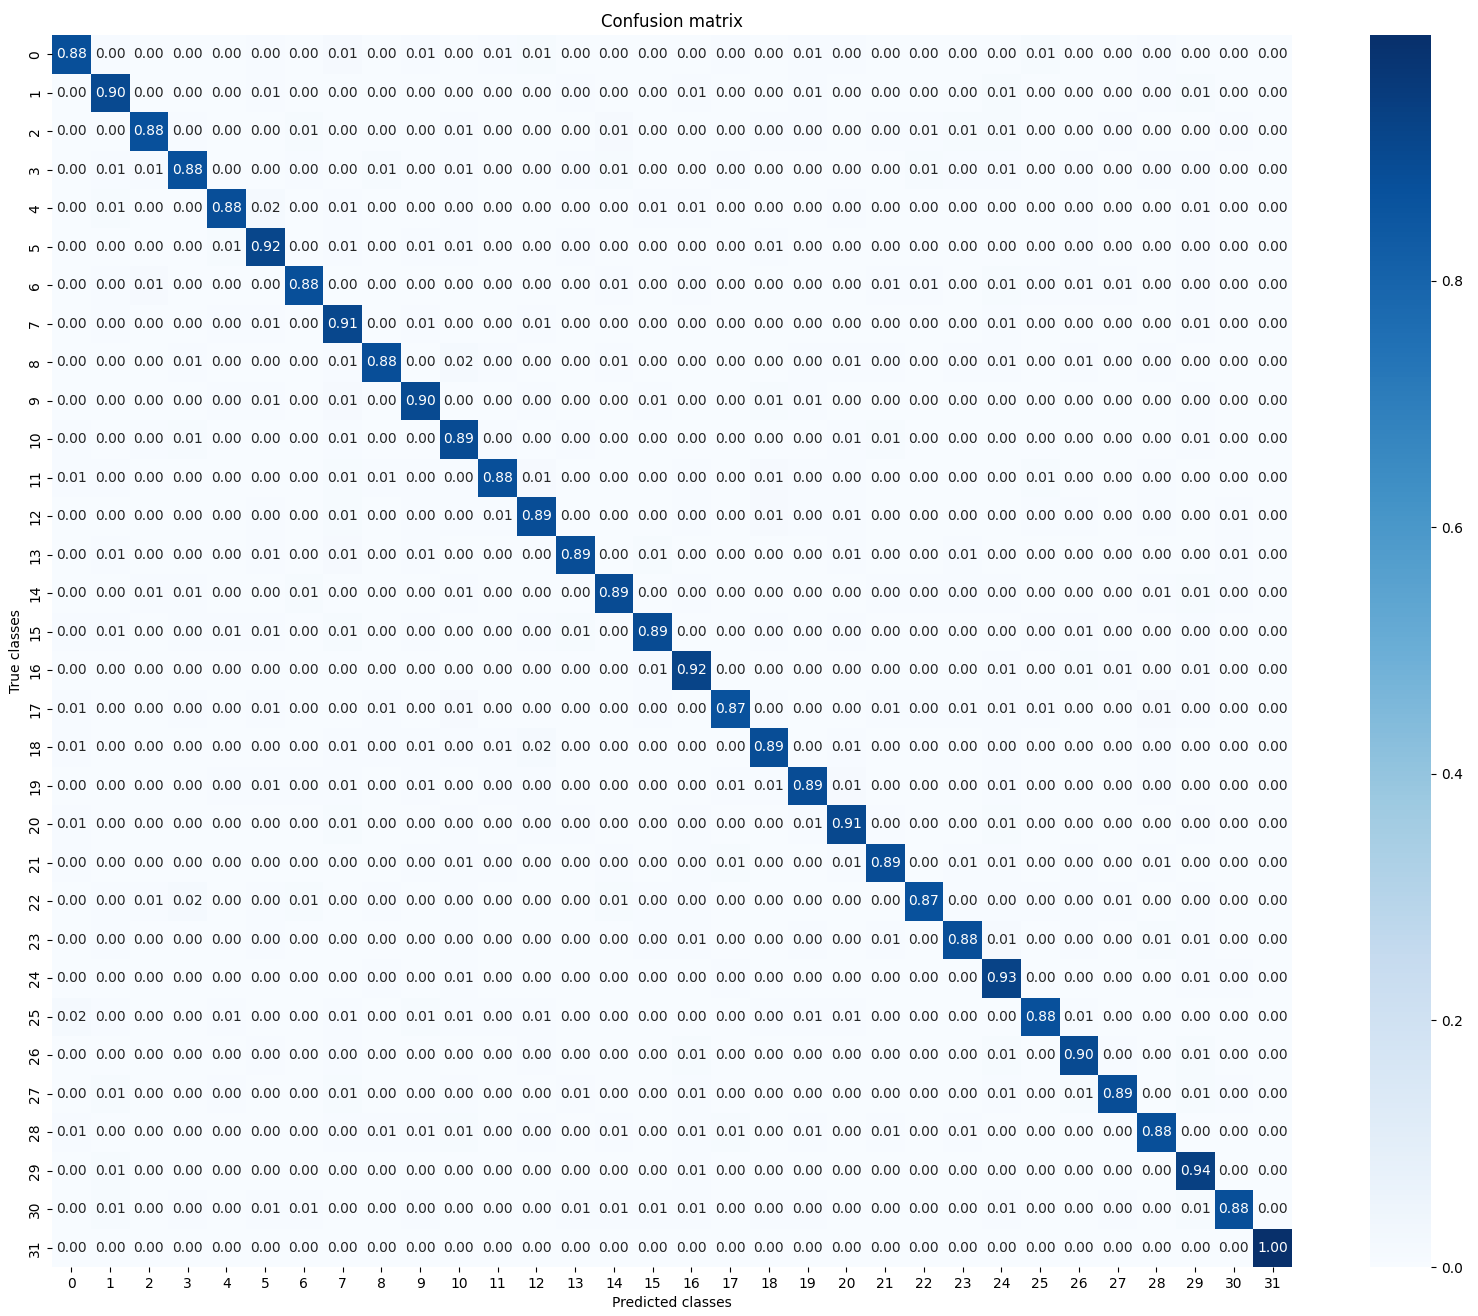
\includegraphics[width=1\linewidth]{imgs/Confusion_matrix.png}
    \caption{Матрица ошибок для обученной Seq-to-Seq модели.}
    \label{fig:cm}
\end{figure}

\vspace{-0.7cm}

Анализ полученных результатов показывает, что точность распознавания последовательностей значительной длины остаётся относительно низкой. Это можно объяснить высокой зависимостью модели Seq-to-Seq от объёма обучающих данных: для эффективного обобщения признаков, извлекаемых из изображений, требуется значительное количество примеров. Следовательно, увеличение размера обучающего набора данных потенциально может способствовать повышению точности модели, однако это также накладывает дополнительные требования к вычислительным ресурсам, необходимым для её обучения.

\chapter*{Заключение}
\addcontentsline{toc}{chapter}{Заключение}

В рамках работы была успешно решена задача автоматизации распознавания текстовых CAPTCHA с применением современных методов машинного обучения. Работа включала в себя как теоретическое обоснование выбранных подходов, так и практическую реализацию нейросетевой модели для решения поставленной задачи.

В ходе исследования были выполнены следующие задачи:

\begin{enumerate}
    \item изучены основные принципы построения текстовых CAPTCHA, включая допустимые символы, типичные искажения, зашумление и методы усложнения распознавания;
    \item проведен анализ существующих архитектур нейронных сетей для задач распознавания последовательностей, в результате чего была выбрана модель типа Seq-to-Seq как наиболее подходящая для условий переменной длины входных последовательностей и сильных искажений;
    \item сформирован и предобработан датасет из 100 000 изображений CAPTCHA, отражающих разнообразие типовых искажений и сложности, присущих реальным CAPTCHA;
    \item реализована процедура обучения нейросетевой модели с использованием библиотеки TensorFlow, обеспечивающая стабильное обучение при различных длинах последовательностей;
    \item проведено тестирование модели на валидационном наборе данных, в ходе которого получена достаточная точность распознавания на последовательностях различной длины, что свидетельствует о пригодности модели для практического применения.
\end{enumerate}

Разработанная модель продемонстрировала способность корректно распознавать текстовые CAPTCHA при наличии значительных искажений и шумов, характерных для реальных сценариев использования. Это подтверждает эффективность предложенного подхода и его применимость в задачах автоматизированного тестирования web-приложений, где необходимость ручного ввода CAPTCHA существенно снижает производительность.

Таким образом, поставленная цель -- разработка и тестирование модели для автоматического распознавания текстовых CAPTCHA -- была достигнута и все запланированные задачи решены. Результаты исследования подтверждают практическую значимость нейросетевых подходов к решению задач подобного рода.

\newpage
\addcontentsline{toc}{chapter}{Список использованной литературы}
\printbibliography[title={Список использованной литературы}]

\appendix
\newpage
\chapter*{\raggedleft\label{appendix1}Приложение}
\phantomsection\addcontentsline{toc}{chapter}{Приложение}

\vspace{-0.5cm}\begin{code}
\captionof{listing}{\label{code:gen-dataset}Исходный код генератора синтетических CAPTCHA}
\vspace{-0.2cm}
{\small
\inputminted[mathescape,linenos,frame=lines,breaklines]{Python}{code/gen-dataset.py}
}
\end{code}

\begin{code}
\captionof{listing}{\label{code:preprocessing}Исходный код для предобработки изображений датасета}
\vspace{-0.5cm}
{\small
\inputminted[mathescape,linenos,frame=lines,breaklines]{Python}{code/preprocessing.py}
}
\end{code}

\begin{code}
\captionof{listing}{\label{code:tf-dataset}Исходный код для создания датасета в формате тензоров}
\vspace{-0.5cm}
{\small
\inputminted[mathescape,linenos,frame=lines,breaklines]{Python}{code/tf-dataset.py}
}
\end{code}

\begin{code}
\captionof{listing}{\label{code:crnn}Исходный код CRNN модели}
\vspace{-0.5cm}
{\small
\inputminted[mathescape,linenos,frame=lines,breaklines]{Python}{code/crnn.py}
}
\end{code}

\begin{code}
\captionof{listing}{\label{code:seq2seq}Исходный код Seq-to-Seq модели}
\vspace{-0.5cm}
{\small
\inputminted[mathescape,linenos,frame=lines,breaklines]{Python}{code/seq-to-seq.py}
}
\end{code}

\begin{code}
\captionof{listing}{\label{code:test-model}Исходный код тестирования Seq-to-Seq модели}
\vspace{-0.5cm}
{\small
\inputminted[mathescape,linenos,frame=lines,breaklines]{Python}{code/test.py}
}
\end{code}

\end{document}
